%\documentclass[12pt]{report}
%\author{Karthik J, Navya Jose}
%\date{}
%\usepackage{../sem12-lab-record}
\lhead{Date: 20/07/2021}
\begin{document}
	
	%\maketitle
	
	\chapter{Inverse Square Law (Beta-radiation)}
	\vspace{-1cm}
	\dateofexp{Date of Experiment: 20/07/2021} 
	% To display date in contents page
	
	\begin{center}% To display date in the experiment page
		Date of Experiment: 20/07/2021
	\end{center}
	\section{Aim}
	To verify inverse square law for beta particles using GM counter.
	
	\section{Requirements}
	\begin{itemize}
		\item 	Geiger M{\"u}ller counter
		\item 	Thallium as beta source
	\end{itemize}

\section{Theory}
For any isotropic emission of radiation from the source the intensity varies inversely as square of the distance from the source. This statement is called the inverse square law. As indicated in the figure, the lines represent the flux lines (lines per unit area) emanating from a point source. The total number of flux lines depends on the strength of the source and is constant at all distances. A greater density of flux lines means a stronger field. The density of flux lines is inversely proportional to the square of the distance from the source because the surface area of a sphere increases with the square of the radius. Thus the strength of the field is inversely proportional to the square of the distance from the source.

Basically inverse square law says that, as the distance between source and detector is doubled, intensity goes down by a factor of four. In general, if the distance increased by $ k $ times, intensity would decrease by a factor of $ k^2 $. As a result, if the source is moved to a distance $ d $ away from the window of the GM counter, then the intensity of radiation decreases by a factor $ 1/d^2 $.


\section{Observations \& Graph}
\noindent
\begin{tabular}{p{0.48\textwidth} p{0.48\textwidth}}
	Operating voltage =  \SI{450}{\volt}&
	Background counts, $ N_b $ = 25
\end{tabular}
\vspace{-10pt}
\begin{table}[h]
	\begin{tabular}{|l|r|r|r|r|r|r|r|}
		\hline
		\rowcolor[HTML]{EFEFEF} 
		\multicolumn{1}{|c|}{\cellcolor[HTML]{EFEFEF}\textbf{Distance}} & \multicolumn{3}{c|}{\cellcolor[HTML]{EFEFEF}\textbf{Count $ (N_i)$}}                                                                                                                              & \multicolumn{1}{c|}{\cellcolor[HTML]{EFEFEF}\textbf{Average }$ N_i $} & \multicolumn{1}{c|}{\cellcolor[HTML]{EFEFEF}$ N = N_i-N_b $} & \multicolumn{1}{c|}{\cellcolor[HTML]{EFEFEF}$ \ln N $} & \multicolumn{1}{c|}{\cellcolor[HTML]{EFEFEF}$ \ln d $} \\ \hline
		\rowcolor[HTML]{EFEFEF} 
		& \multicolumn{1}{c|}{\cellcolor[HTML]{EFEFEF}\textbf{Trial 1}} & \multicolumn{1}{c|}{\cellcolor[HTML]{EFEFEF}\textbf{Trial 2}} & \multicolumn{1}{c|}{\cellcolor[HTML]{EFEFEF}\textbf{Trial 3}} & \multicolumn{1}{l|}{\cellcolor[HTML]{EFEFEF}}                    & \multicolumn{1}{l|}{\cellcolor[HTML]{EFEFEF}}                   & \multicolumn{1}{l|}{\cellcolor[HTML]{EFEFEF}}              & \multicolumn{1}{l|}{\cellcolor[HTML]{EFEFEF}}              \\ \hline
		3.3                                                             & 116,350                                                       & 116,692                                                       & 117,055                                                       & 116,699                                                          & 116,674                                                         & 11.67                                                      & 1.19                                                       \\ \hline
		4.3                                                             & 99,241                                                        & 99,049                                                        & 99,502                                                        & 99,264                                                           & 99,239                                                          & 11.51                                                      & 1.46                                                       \\ \hline
		5.3                                                             & 79,084                                                        & 79,080                                                        & 79,059                                                        & 79,074                                                           & 79,049                                                          & 11.28                                                      & 1.67                                                       \\ \hline
		6.3                                                             & 61,979                                                        & 62,315                                                        & 62,128                                                        & 62,141                                                           & 62,116                                                          & 11.04                                                      & 1.84                                                       \\ \hline
		7.3                                                             & 50,490                                                        & 50,382                                                        & 50,116                                                        & 50,329                                                           & 50,304                                                          & 10.83                                                      & 1.99                                                       \\ \hline
		8.3                                                             & 39,799                                                        & 39,899                                                        & 39,911                                                        & 39,870                                                           & 39,845                                                          & 10.59                                                      & 2.12                                                       \\ \hline
		9.3                                                             & 33,370                                                        & 33,399                                                        & 33,399                                                        & 33,389                                                           & 33,364                                                          & 10.42                                                      & 2.23                                                       \\ \hline
		10.3                                                            & 27,763                                                        & 27,722                                                        & 27,931                                                        & 27,805                                                           & 27,780                                                          & 10.23                                                      & 2.33                                                       \\ \hline
		11.3                                                            & 23,830                                                        & 23,843                                                        & 23,732                                                        & 23,802                                                           & 23,777                                                          & 10.08                                                      & 2.42                                                       \\ \hline
		12.3                                                            & 20,769                                                        & 20,810                                                        & 20,661                                                        & 20,747                                                           & 20,722                                                          & 9.94                                                       & 2.51                                                       \\ \hline
		13.3                                                            & 17,995                                                        & 17,992                                                        & 17,998                                                        & 17,995                                                           & 17,970                                                          & 9.80                                                       & 2.59                                                       \\ \hline
	\end{tabular}
\caption{Observations}
\label{tab:1202-obs}
\end{table}
%


\begin{figure}[!htb]
	\centering
	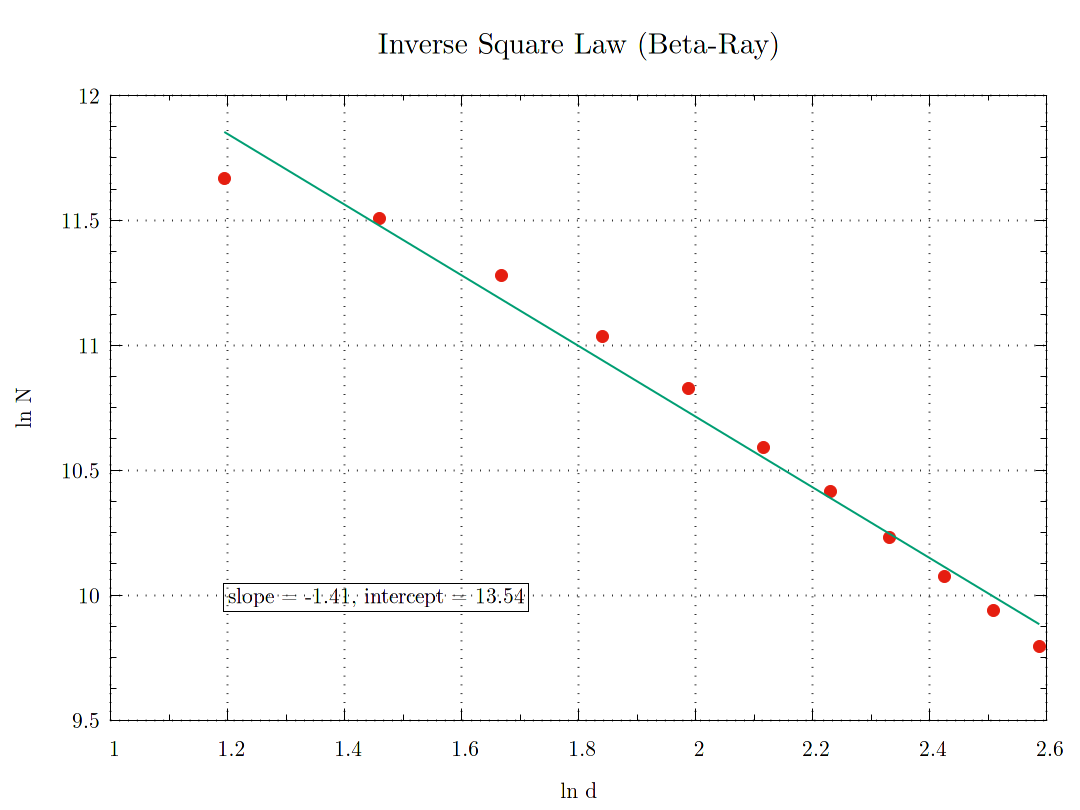
\includegraphics[width=0.7\linewidth]{Experiments/1202-plot}
	\caption{Plot of $ \ln N $ versus $ \ln d $}
	\label{fig:1202-plot}
\end{figure}



\section{Result}

\end{document}
